\section{Имитационное моделирование}
В данной работе анализ полученных асимптотических результатов для систем массового обслуживания с повторными вызовами и вызываемыми заявками проводится с использованием имитационного моделирования. Построив имитационную модель системы, мы получаем возможность провести численное сравнение результатов ее работы с аналитическим решением для оценки его применимости на практике.

Имитационное моделирование систем массового обслуживания \cite{wieland2003queueing} сводится к генерированию случайных времен с соответствующим распределением вероятности, по прошествии которого в системе наступит некоторое событие --- приход заявки, окончание обслуживания и т.д., что называется дискретно--событийным подходом. Таким образом, в течение моделирования на протяжении некоторого заданного времени модель обрабатывает происходящие в системе события --- они регистрируются, и на их основе подсчитываются численные характеристики, такие как распределение вероятности.

Реализованная имитационная модель, как программный продукт, разрабатывалась с возможностью расширения ее функционала для предоставления возможности тонко настраивать параметры моделирования и без препятствий извлекать полученные результаты в виде распределения вероятности для последующего анализа. В этих целях, программа реализована при помощи объектно--ориентированного подхода, так как данный подход позволил выстроить логику работу программы на уровне абстракций, что и дает возможность легкого расширения функционала и реализации моделей других систем массового обслуживания.

\subsection {Объектная модель предметной области}
Для построения объектной модели предметной области программы рассматриваются следующие объекты систем массового обслуживания, используемые в данной работе:
\begin{itemize}
\item Заявка --- объект, который поступает в систему, перемещается по ней и , в конечном итоге, покидает систему в течение моделирования.
\item Обслуживающий прибор --- объект, принимающий на вход заявки и обслуживающий их. По окончании обслуживания заявки покидают прибор.
\item Орбита --- скопление заявок, ожидающих повторного обращения на обслуживающий прибор.
\item Входящий поток --- объект, генерирующий заявки, которые поступают на прибор.
	\end{itemize}
 Поскольку процесс работы модели заключается в перемещении заявок по системе, то в некоторый момент времени моделирования $T_{cur}$ местонахождение каждой заявки и ее характеристики могут меняться. В таком случае, необходимо отслеживать момент времени, в который заявка изменит свое состояние --- $T_{shift}$. В момент времени, когда $T_{shift} = T_{curr}$,  происходит смена состояния заявки, и  $T_{shift}$ обновляется объектом системы массового обслуживания, в которой она на данный момент находится. Среди событий , при которых происходит обновление момента смены состояния заявки, выделим следующие:
\begin{itemize}
	\item Заявка покидает входящий поток --- в данном случае в источнике генерируется новая заявка с моментом времени $T_{shift}$, при наступлении которого, она также покинет входящий поток.
	\item Заявка успешно поступила на прибор и начала обслуживаться --- в этом случае обслуживающий прибор определяет для заявки момент времени $T_{shift}$, в который ее обслуживание закончится.
	\item При попытке поступить на прибор заявка застала его занятым обслуживанием другой заявки и отправилась на орбиту. По прибытии на орбиту, новый момент времени $T_{shift}$ заявки определяется как время, при наступлении которого заявка покинет орбиту.
\end{itemize}
Исходя из вышеописанного, центральными объектами в предметной области являются заявка и событие, наступающее в системе при смене состояния заявки. В предметной области они представлены классом Event, который связан ассоциацией с перечислением EventType, элементы которого соответствуют объектам системы обслуживания, в которых наступило  событие. Это позволяет собирать статистику о произошедших событиях в системе.
\begin{figure}[H]
	\centering
	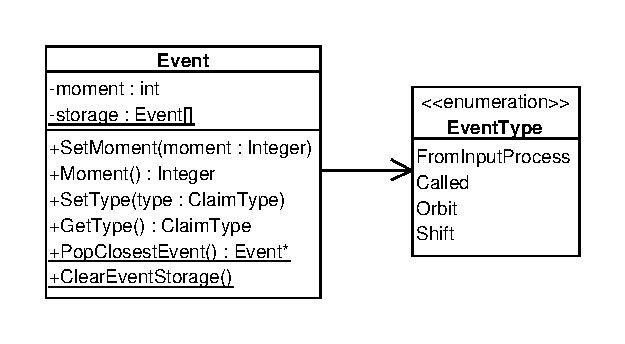
\includegraphics[scale=1]{event_uml.eps}
	\caption{Класс Event}
	\label{event_uml}
\end{figure}
Поле moment хранит момент времени $T_{shift}$ до изменения состояния объекта. Для того, чтобы определить, какое событие должно произойти в модели следующим, класс Event содержит статическую коллекцию собственных объектов --- storage. При создании новых событий они также помещаются и в storage для того, чтобы в последствии извлекать следующее по времени событие c помощью метода PopClosestEvent.

Для реализации подхода, основанном на постоянном обновлении состоянии заявок, находящихся в системе, предметная область базируется на общем интерфейсе, который реализуют все конкретные элементы рассматриваемых систем массового обслуживания. Его цель заключается в формализации изменения состояния элемента системы с каждым промежутком времени, в течение которого наступило очередное событие. Поскольку, сам класс RQ--системы, как будет показано ниже, реализует данный интерфейс, то возможно использовать ее как входящий поток для другой системы.
\begin{figure}[H]
	\centering
	
\includegraphics[scale=1]{processable_uml.eps}
	\caption{Общий интерфейс Processable для всех элементов системы массового обслуживания}
	\label{processable_uml}
\end{figure}
Метод Process унифицирует все изменения в элементе системы массового обслуживания, которые должны произойти в нем при наступлении события. Реализация этого интерфейса не обязательно должна иметь только этот метод, так как для удобства организации логики работы элемента, удобно размещать некоторые алгоритмы в отдельным методах.

Также, не все элементы системы можно полностью описать данным интерфейсом --- обслуживающий прибор и орбита, помимо общего метода Process, должны иметь точки входа для заявок. По этой причине для них определены соответствующие интерфейсы, наследуемые от Processable.
\begin{figure}[H]
	\centering
	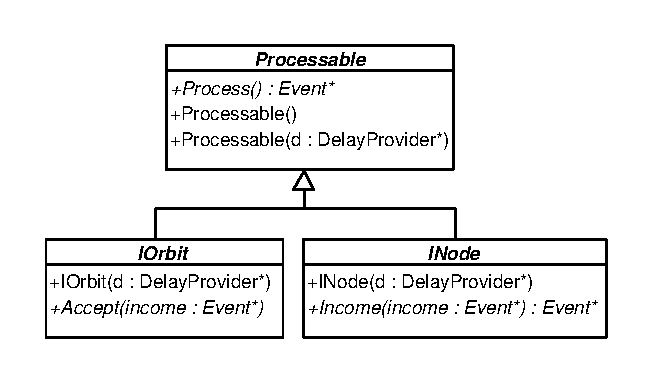
\includegraphics[scale=1]{inode_iorbit_uml.eps}
	\caption{Интерфейсы для обслуживающего прибора (INode) и орбиты (IOrbit), наследуемые от Processable}
	\label{inode_iorbit_uml}
\end{figure}
Метод IOrbit Accept служит для принятия заявок на орбиту, а метод INode Income --- для принятия заявки на прибор для обслуживания. Отличие между данными методами заключается в том, что, если прибор занят обслуживанием другой заявки, то метод Income вернет заявку, которая пытается встать на прибор, в то время как орбита не имеет ограничения по количеству находящихся на ней заявок.

Для вычисления экспоненциальной задержки до наступления событий в модели, в предметную область был добавлен общий интерфейс для объектов, вычисляющих задержку, что позволяет менять способ вычисления задержки в процессе моделирования.
\begin{figure}[H]
	\centering
	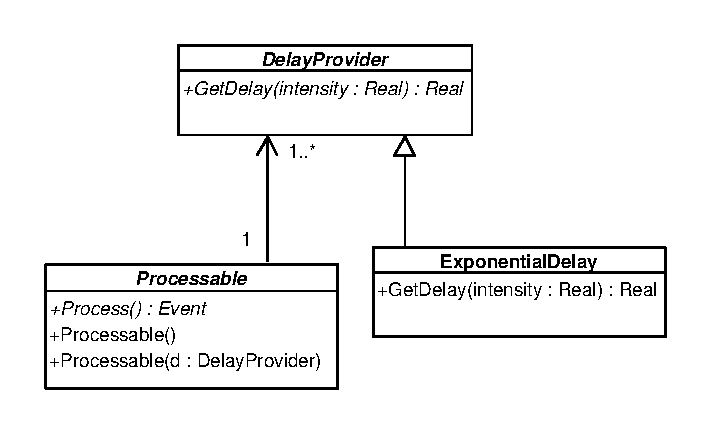
\includegraphics[scale=1]{delayprovider_uml.eps}
	\caption{DelayProvider --- интерфейс для вычисления задержки, который используют элементы системы массового обслуживания}
	\label{delayprovider_uml}
\end{figure}

Для обеспечения среды, которой будет происходит моделирование, а именно --- вестись подсчет прошедшего времени, взаимодействие с реализацией интерфейса Processable и сбор статистики, введен глобальный объект Environment
\begin{figure}[H]
	\centering
	
\includegraphics[scale=1]{environment_uml.eps}
	\caption{Глобальный объект Environment}
	\label{environment_uml}
\end{figure}

Статический класс Environment содержит общую для модели информацию --- время моделирования, время конца моделирования и методы, для управления этими параметрами. 
Члены класса Environment будут описаны в последующих разделах.

\begin{figure}[H]
	\centering
	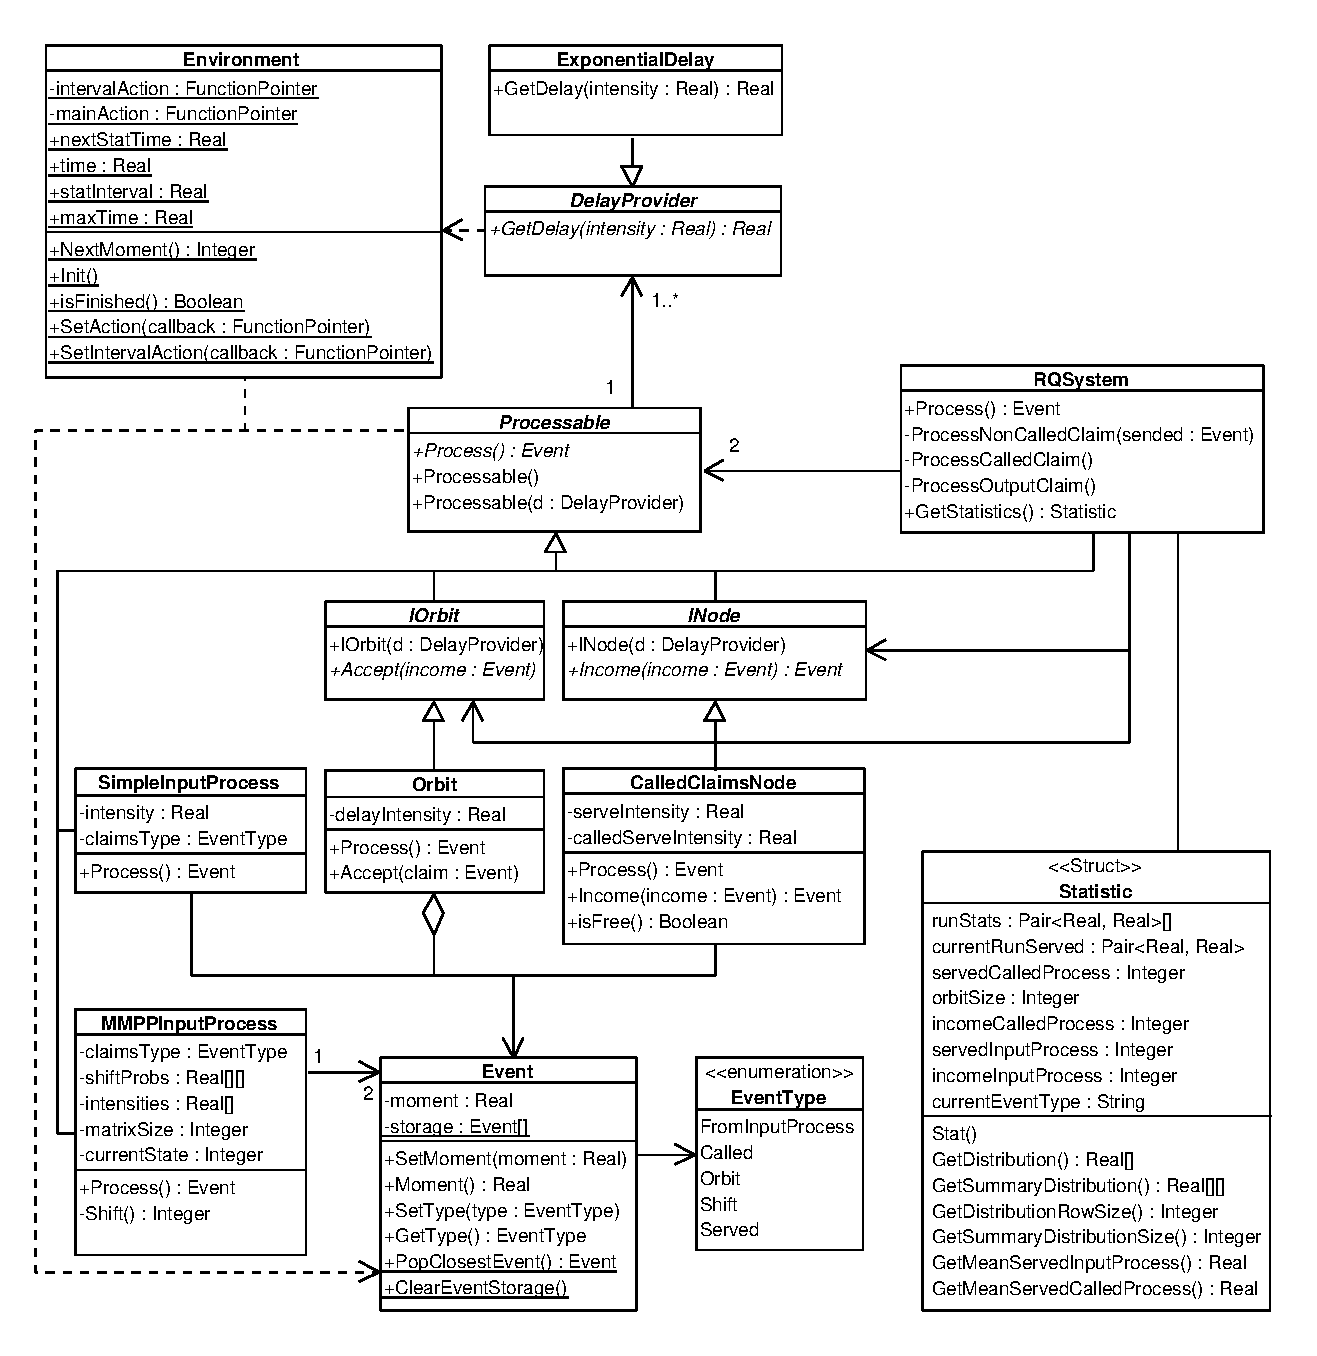
\includegraphics[scale=0.79,width=\textwidth]{domain_uml.eps}
	\caption{Предметная область имитационной модели}
	\label{domain_uml}
\end{figure}
На рисунке \ref{domain_uml} представлена полная предметная область программы. Определенные ранее интерфейсы реализуют конкретные элементы системы, используемые при моделировании. Поскольку, в данной работе рассматривается RQ--система с простейшим и MMPP--потоками, существует две соответствующих реализации входящего потока, подробности функционирования которых будут рассмотрены в следующем разделе. Таким образом, существуют следующие реализации элементов систем массового обслуживания:
\begin{itemize}
	\item Orbit --- реализация источника повторных вызовов, содержащая хранилище заявок (Event), что на диаграмме классов показано агрегацией. Поле delayIntensity хранит интенсивность обращений заявок с орбиты, то есть используется для вычисления экспоненциальной задержки соответствующим объектом DelayProvider.
	\item CalledClaimsNode --- реализация обслуживающего прибора, способная обслуживать два типа заявок --- пришедшие извне и вызванные, для чего служат интенсивности serveIntensity и calledServeIntensity соответственно.
	\item SimpleInputProcess --- реализация простейшего входящего потока, порождающего заявки. Ассоциация с Event показывает, что класс имеет поле с заявкой, которая готовится покинуть источник заявок по истечении задержки.
	\item MMPPInputProcess --- реализация MMPP-потока. Поле shiftProbs хранит матрицу интенсивностей переходов между состояниями, а поле intensities --- интенсивность поступления заявок для каждого состояния. Логика смены состояний находится в приватном методе Shift, где используются поле currentState --- номер текущего состояния, а так же объект Event, в котором хранится момент сменты состояния входящего потока, что на диаграмме показано ассоциацией с множителем 2.
	\item RQSystem представляет агрегирующий класс, где при помощи описанных выше классов строится логика работы системы.
	\item Структура Statistic служит для сбора и подсчета различных характеристик системы в процессе моделирования --- одномерного и двумерного распределения, математического ожидания и др. 
\end{itemize}
\clearpage
\subsection{Процесс моделирования}
В качестве среды для моделирования в реализованной программе выступает глобальный объект Environment, представленный на рисунке \ref{environment_uml}. В процессе моделирования у него вызывается метод NextMoment, который переносит систему в следующий момент моделирования, то есть, совершается одна итерация процесса моделирования. Перед началом моделирования вызывается метод Init, который подготавливает модель к началу работы. Метод isFinished служит для осведомления других участков программы, что моделирование окончено, то есть, что выставленное время моделирования (maxTime) равно текущему (time).

Для обеспечения гибкости действий, которые модель может совершать в процессе работы, метод NextMoment имеет частичную реализацую, в которой вызывается указатель на функцию или лямбда--выражение mainAction. Таким образом, поведение модели можно менять в процессе ее работы, что делает класс Environment универсальным для многих систем, использующих пошаговое моделирование.
\begin{figure}[H]
	\centering
	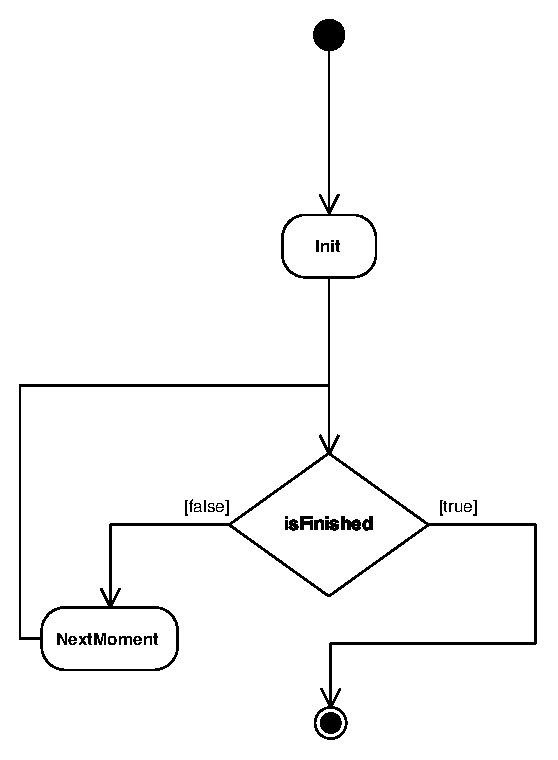
\includegraphics[scale=0.75]{simulation_algo_uml.eps}
	\caption{Общий алгоритм процесса моделирования на основе класса Environment}
	\label{simulation_algo_uml}
\end{figure}

Для сбора статистики и построения распределения вероятностей количества обслуженных заявок в классе Environment предусмотрен механизм интервального сбора данных. Поле statInterval хранит интервал модельного времени, по прошествии которого должен производится вызов функции или лямбда выражения по указателю intervalAction, в котором задается логика сбора данных.

Как видно на рисунке \ref{domain_uml}, класс Environment зависит от класса Event, так как в нем содержится статистическая очередь событий storage, которые вскоре должны произойти в системе. Наглядно это показано на диаграмме последовательностей:
\begin{figure}[H]
	\centering
	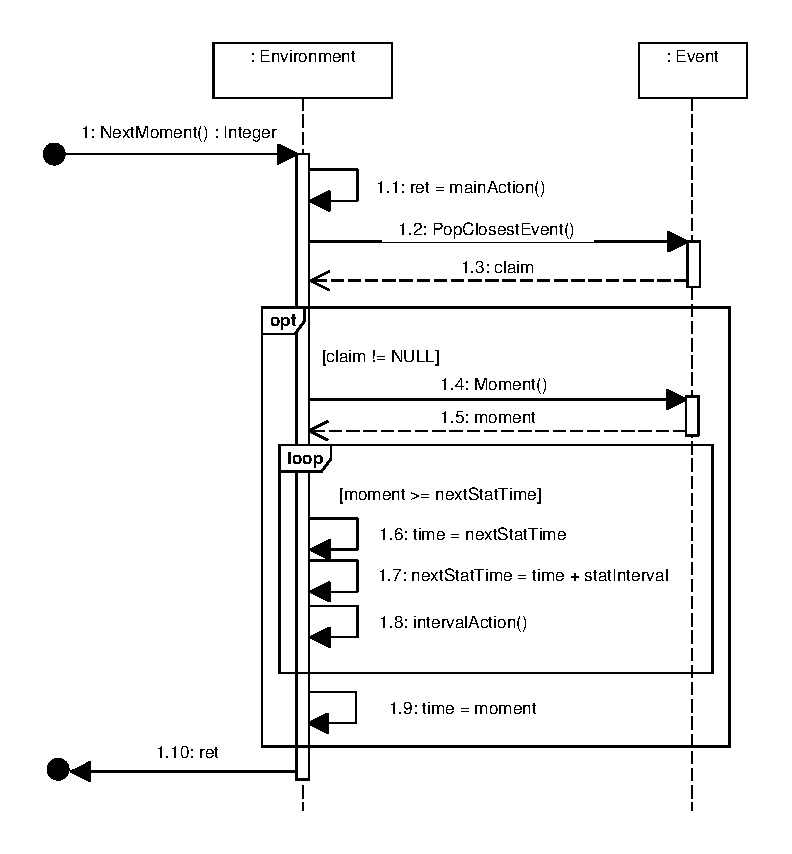
\includegraphics[scale=0.9]{next_moment_algo_uml.eps}
	\caption{Диаграмма последовательностей метода NextMoment}
	\label{next_moment_algo_uml}
\end{figure}
После выполнения mainAction (1.1), из очереди событий извлекается первое предстоящее (1.2). Если такое нашлось, то модельное время перемещается на момент события (1.9). Если это время больше, чем время сбора статистики, то сначала выполняется сбор (1.8), и уже после этого модельное время смещается на момент события. Сбор статистики выполняется в цикле, так как время наступления события может быть больше интервала сбора статистики в несколько раз.
\clearpage
\subsection{Функционирование элементов системы массового обслуживания}
Функционирование же отдельных элементов системы описывается в методах интерфейса Processable и наследуемых от него INode и IOrbit.
Происходящее с обслуживающим прибором во время очередной итерации отражено на диаграммах последовательностей \ref{CalledClaimsNode_Process_uml} и \ref{CalledClaimsNode_Income_uml}
\begin{figure}[H]
	\centering
	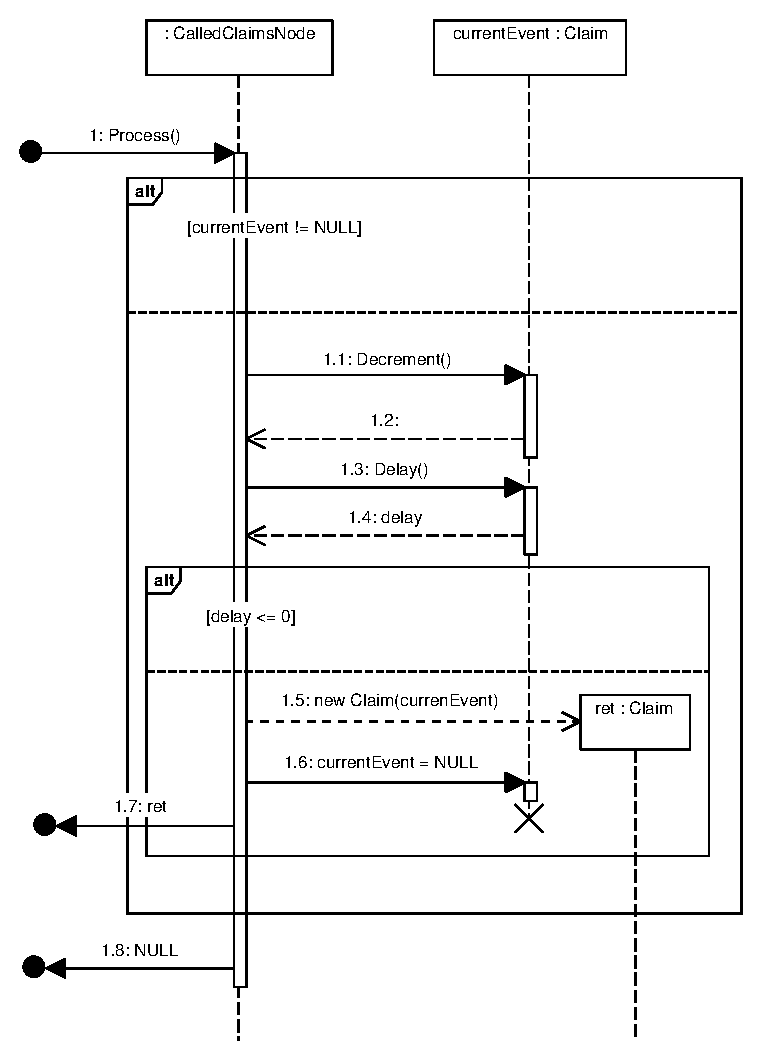
\includegraphics[scale=0.9]{CalledClaimsNode_Process.eps}
	\caption{Диаграмма последовательностей метода Process класса CalledClaimsNode}
	\label{CalledClaimsNode_Process_uml}
\end{figure}
Если прибор на данный момент не обслуживает заявку currentEvent (поле currentEvent на диаграмме \ref{domain_uml} обозначено ассоциацией), то возвращается NULL, говорящий о том, что на данной итерации прибор не закончил обслуживание заявки, так как он либо свободен, либо обслуживание еще продолжается. Иначе, производится проверка, совпадает ли текущее модельное время с моментом наступления события. При совпадении обслуженная заявка уходит с прибора (1.5, 1.6, 1.8).
\begin{figure}[H]
	\centering
	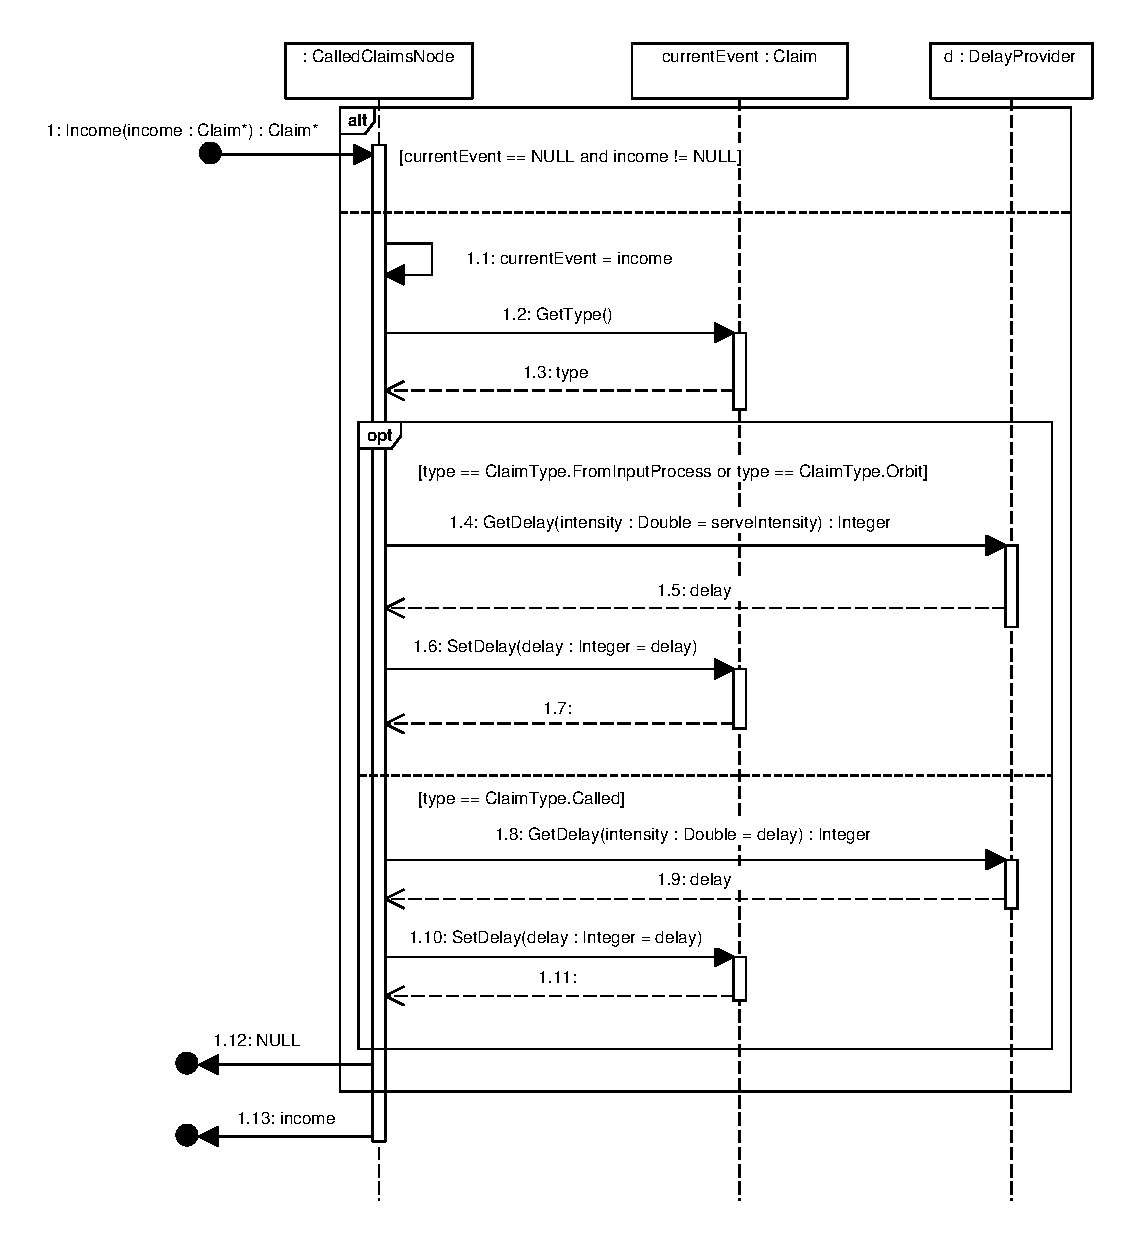
\includegraphics[scale=0.9]{CalledClaimsNode_Income.eps}
	\caption{Диаграмма последовательностей метода Income класса CalledClaimsNode}
	\label{CalledClaimsNode_Income_uml}
\end{figure}
В случае, если пришла заявка, и прибор свободен, пришедшая заявка становится текущей обслуживаемой на приборе (1.1), иначе она возвращается (1.13). В зависимости от типа пришедшей заявки для нее вычисляется время обслуживания --- для заявок с входящего потока и орбиты используется serveIntensity (1.4, 1.6), а для  вызванных используется calledServeIntensity (1.8, 1.10).

Подобный алгоритм, заключающийся в сравнении модельного времени с моментом наступления события, реализован и в других элементах системы.
В методе Accept класса Orbit также вычисляется задержка для пришедшей заявки. После чего она помещается в коллекцию claimStorage, отображенной на диаграмме предметной области (рисунок \ref{domain_uml}) в качестве агрегации. В методе Process (рисунок \ref{Orbit_Process_uml}) производится обход данной коллекции со сравнением времени, когда заявка должна покинуть орбиту, и модельным временем. В случае, если нашлась готовая заявка, она извлекается (1.5) из коллекции и возвращается (1.6).
 \begin{figure}[H]
 	\centering
 	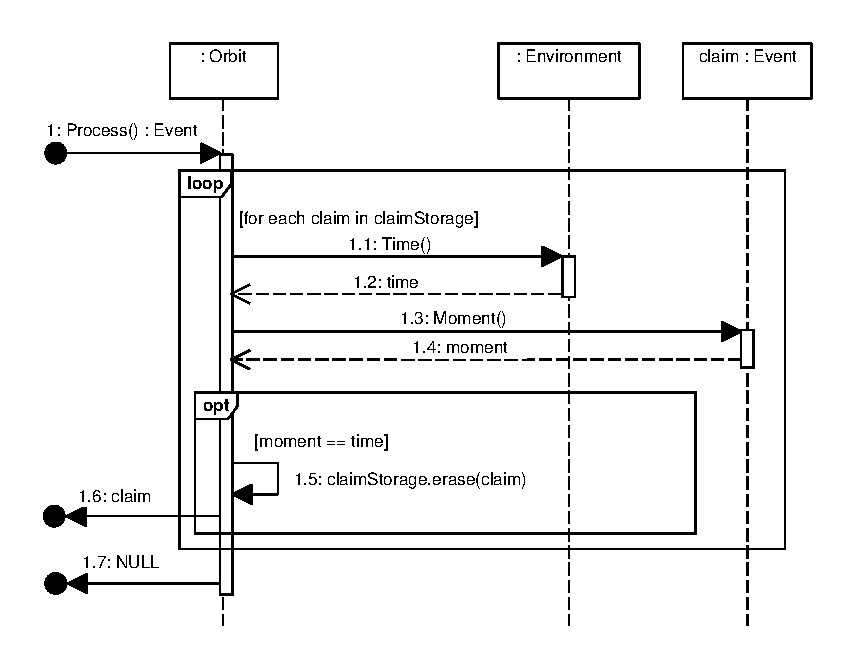
\includegraphics[scale=0.9]{Orbit_Process.eps}
 	\caption{Диаграмма последовательностей метода Process класса Orbit}
 	\label{Orbit_Process_uml}
 \end{figure}
Тот же подход используется для метода Process классов SimpleInputProcess и \\ MMPPInputProcess. Более подробного рассмотрения требует алгоритм смены состояния управляющей цепи MMPP--потока, реализованного в методе Shift класса MMPPInputProcess.

Как было показано в главе \ref{mmpp_section}, время нахождения в одном из состояний и вероятность перехода в другое для MMPP-потока определяется матрицей инфинитезимальных характеристик $Q$
\begin{equation*}
	\boldsymbol{Q}=\begin{bmatrix}
		q_{11} &  \dots &  q_{1n}\\
		\vdots & \ddots &  \\
		q_{n1} &    	&	q_{nn}
	\end{bmatrix}
\end{equation*}
Интенсивностью, на основе которой вычисляется задержка управляющей цепи в $i$--ом состоянии является диагональный элемент матрицы $-q_{i,i}$, а вероятностью перехода из $i$--ого состояния в $j$--ое является выражение $\frac{q_{i,j}}{-q_{i,i}}$.В таком случае, при наступлении события смены состояния выполняется следующий алгоритм
   \begin{figure}[H]
  	\centering
  	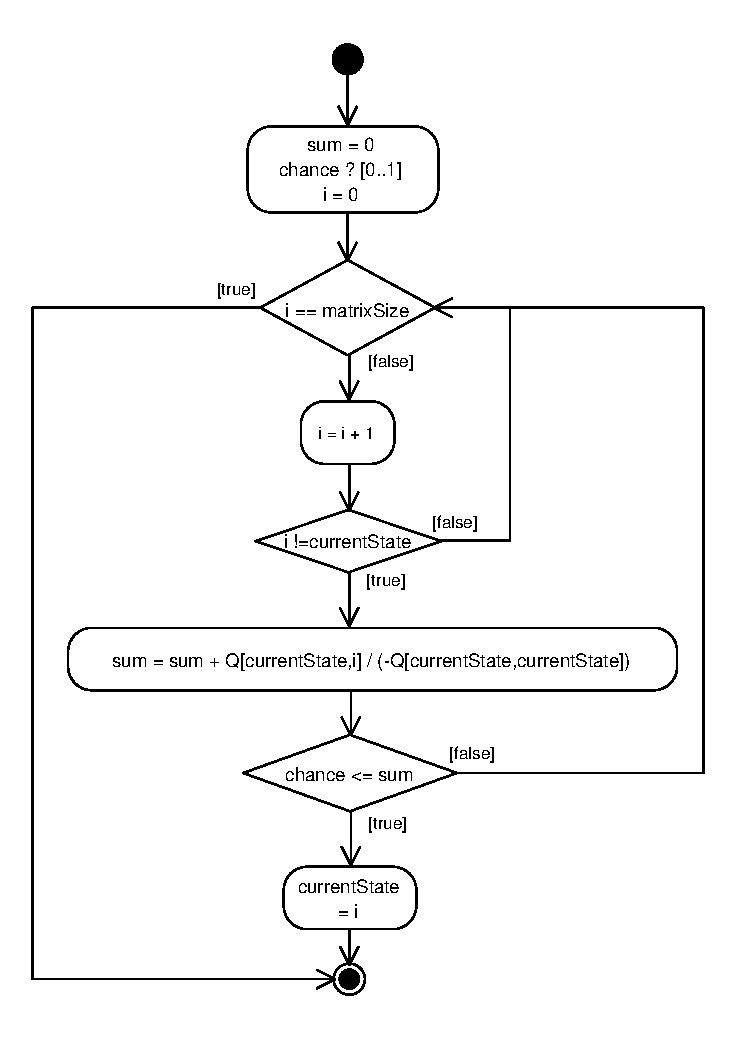
\includegraphics[scale=0.7]{shift_algo.eps}
  	\caption{Алгоритм смены состояния MMPP--потока}
  	\label{shift_algo_uml}
  \end{figure}
В начале работы вычисляется случайная величина chance, определяется переменная sum для суммирования вероятностей по строке матрицы $Q$ и счетчик цикла i. Цикл идет по строке текущего состояний currentState. В случае, если текущий элемент строки недиагональный, к sum прибавляется вероятность попадания в состояние i, после чего производится проверка, больше ли величина sum случайной величины chance. Графически это представляется таким образом, что точка chance принадлежит отрезку $[0,sum]$, а прибавленная к sum на текущей итерации вероятность попадания управляющей цепи в состояние i обеспечила принадлежность точки к отрезку, следовательно, прибор принимает состояние i. После этого время нахождения управляющей цепи в нем рассчитывается с помощью метода GetDelay интерфейса DelayProvider.
\clearpage
\subsection{Интерфейс и работа программы}
Для начала работы с программой, в первую очередь, необходимо задать параметры моделирования. Среди них:
\begin{itemize}
	\item Время моделирования (Time limit). Данные единицы являются условными и используются в качестве модельного времени.
	\item Тип входящего потока (Input Process).
	\item Интенсивность входящего потока (Simple input). Для MMPP--потока матрица инфинитезимальных характеристик и вектор интенсивностей задается в модельном окне.
	\item Интенсивность вызова заявок прибором (Calling intensity).
	\item Интенсивность обслуживания входящих и вызванных заявок (Serving intensity, Called serving intensity).
	\item Интервал сбора статистики для построения распределения вероятностей (Moment T). Так же выражен в единицах модельного времени.
\end{itemize}
   \begin{figure}[H]
	\centering
	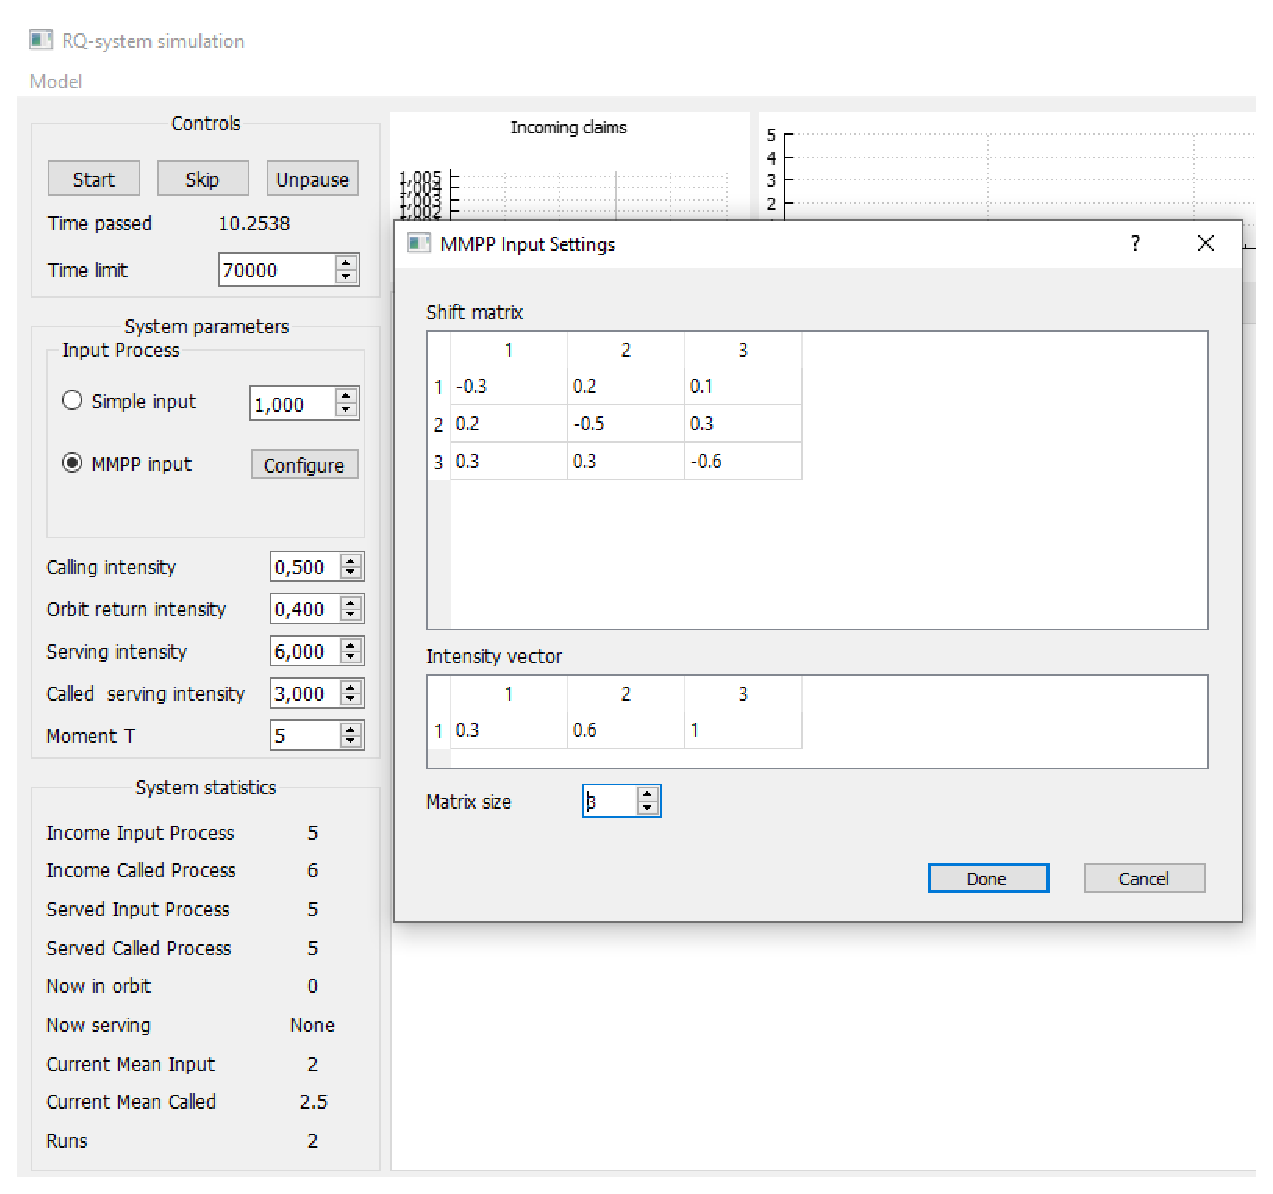
\includegraphics[scale=0.5]{interface_params.eps}
	\caption{Задание параметров моделирования}
	\label{interface_params}
\end{figure}
Управление процессом моделирования выполняется с помощью специальной области Controls (рисунок \ref{interface_params}). Кнопка Start сбрасывает результаты предыдущего запуска модели и начинает моделирование заново с установленными параметрами.
\subsubsection{Моделирование в реальном времени}
Реализация программы предусматривает два варианта работы с моделью. В первом случае, пользователь имеет возможность в реальном времени наблюдать, как меняется состояние системы с помощью визуализации распределения вероятностей числа обслуженных заявок и других характеристик на графиках и в области System statistics, а также приостанавливать моделирование с помощью кнопки Pause, которая так же служит и для возобновления процесса моделирования. Данный подход реализован с помощью таймера, при каждом тике которого выполняется очередная итерация моделирования. Для настройки длины интервала таймера используется модальное окно конфигурации:
\begin{figure}[H]
	\centering
	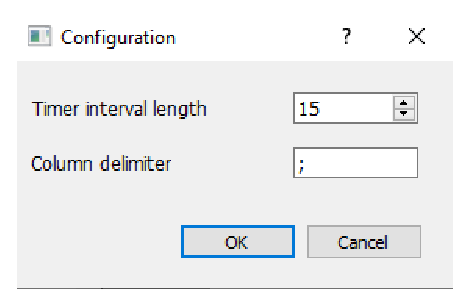
\includegraphics[scale=0.7]{interface_config.eps}
	\caption{Модальное окно конфигурации}
	\label{interface_config}
\end{figure}
Измененные пользователем настройки сохраняются в файле конфигурации для использования их в последующих запусках программы. Предназначение второго параметра будет описано в следующих разделах.

   \begin{figure}[H]
	\centering
	\includegraphics[scale=0.5,width=\textwidth]{interface_realtime.eps}
	\caption{Моделирование работы системы в реальном времени}
	\label{interface_realtime}
\end{figure}
Как видно на рисунке \ref{interface_realtime}, в момент, когда в системе наступает очередное событие, то есть, ее состояние меняется, производится сбор статистики и ее показ в реальном времени. Основная статистика работы модели показана в области System statistics, которая содержит следующую информацию:
\begin{itemize}
	\item Количество пришедших заявок входящего потока (Income Input Process).
	\item Количество заявок, вызванных прибором (Income Called Process).
	\item Количество обслуженных заявок входящего потока (Served Input Process).
	\item Количество обслуженных вызванных прибором заявок (Served Called Process).
	\item Количество заявок на орбите в данный момент (Now in orbit).
	\item Тип в данный момент обслуживаемой заявки (Now serving).
	\item Математическое ожидание обслуженных заявок входящего потока (Current Mean Input).
	\item Математическое ожидание обслеженных вызванных прибором заявок (Current Mean Called).
	\item Количество сборов статистики, интервал которых задан параметром Moment T (Runs).
\end{itemize}
Поскольку математическое ожидание вычисляется на основе полученного на данный момент распределения вероятности, обновление полей Current Mean Input и Current Mean Called происходит с интервалом Moment T. Для отображения области System statistics используется ранее упомянутая структура Statistic (рисунок \ref {domain_uml}), которая служит для накопительного сбора статистики и подсчета распределения и математического ожидания. 

Помимо текстового представления, изменение состояния системы отражено на графиках. Левый верхний график отображает моменты поступления заявок входящего потока. По оси X отсчитывается модельное время.
   \begin{figure}[H]
	\centering
	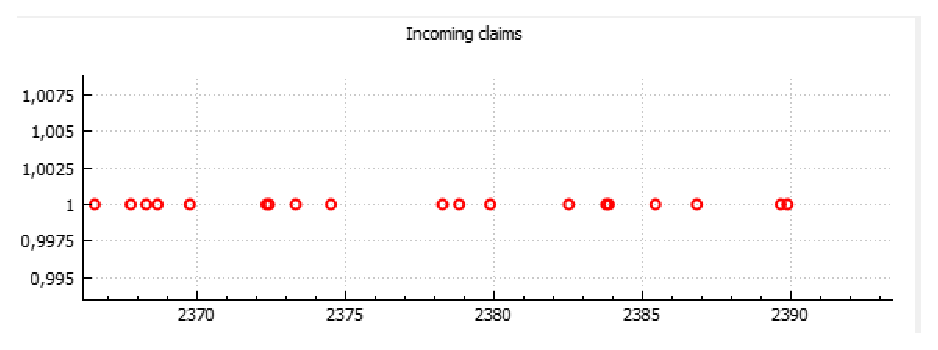
\includegraphics[scale=0.7]{incoming_claims.eps}
	\caption{Отображение времени прихода заявок в систему на графике}
	\label{interface_incoming_claims}
\end{figure}
Правый верхний график отображает изменение количества заявок на орбите в случае моделирования системы с простейшим входящим потоком и историю изменения состояния управляющей цепи MMPP--потока при моделировании системы с MMPP--потоком. По оси X для обоих графиков отсчитывается модельное время. По оси Y количество заявок на орбите, либо состояние управляющей цепи.

   \begin{figure}[H]
	\centering
	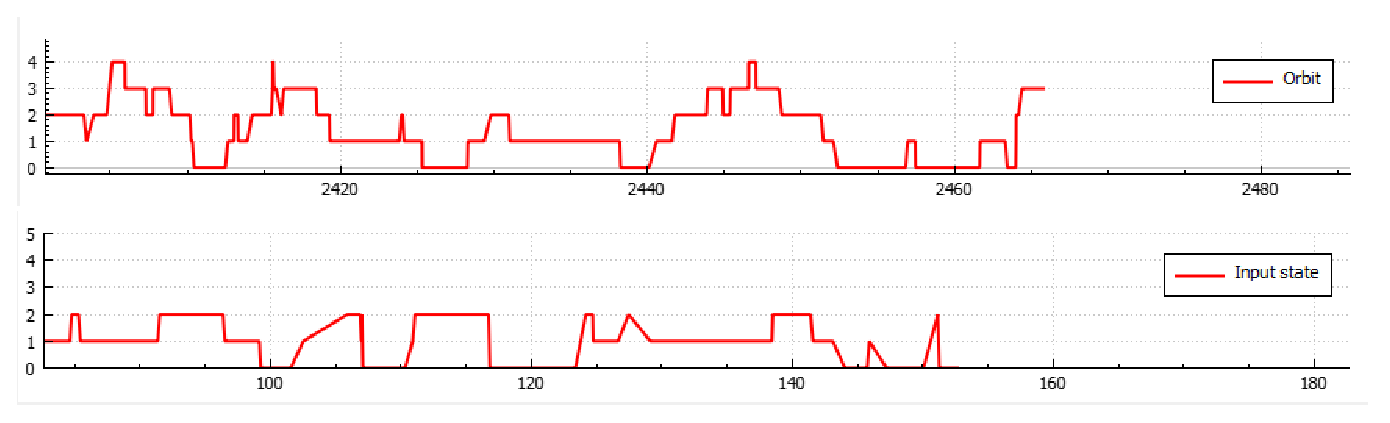
\includegraphics[scale=0.8,width=\textwidth]{orbit_mmppState.eps}
	\caption{Отображение изменения размера орбиты (верхний) и состояния управляющей цепи (нижний) на графике}
	\label{interface_orbit_mmpp}
\end{figure}
Графики на рисунках \ref{interface_incoming_claims} и \ref{interface_orbit_mmpp} имеют опцию масштабирования к выделенной пользователем области.
\subsubsection{Ускоренное моделирование }
Второй вариант работы с программой предполагает, что пользователю требуется быстро получить результаты моделирования. Для этого служит кнопка Skip в области Controls, при нажатии которой таймер останавливается, и производится моделирование системы до установленного времени в цикле. В таком случае, программа отобразит модальное окно, уведомляющее пользователя, что на данный момент выполняется моделирование, блокируя основное.
 \begin{figure}[H]
	\centering
	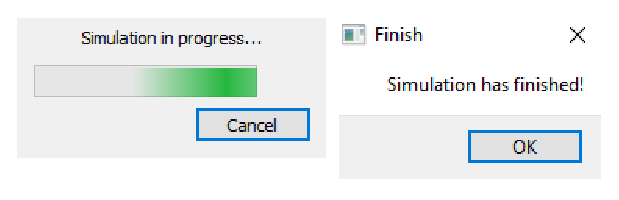
\includegraphics[scale=0.84]{interface_skip.eps}
	\caption{Модальные окна уведомления пользователя о статусе процесса моделирования}
	\label{interface_skip}
\end{figure}
По завершении моделирования отображаемая статистика и главный график обновляются в соответствии с актуальными результатами. По нажатии кнопки отмены (Cancel) в модальном окне статуса моделирования цикл закончит свою работу, а таймер возобновит отсчет. Таким образом, программа продолжит моделирование в реальном времени.  
\subsubsection{Работа с главным графиком}
Важнейшую информацию о работе системы отображает главный график, занимающий наибольшую рабочую область окна. На нем отображается текущее двумерное распределение вероятностей числа обслуженных заявок входящего потока и вызванных заявок в виде трехмерных столбцов. Распределение обновляется в момент модельного времени, кратный параметру Moment T. По осям X и Y отложены количество обслуженных заявок входящего потока и вызванных заявок соответственно.
\begin{figure}[H]
	\centering
	\includegraphics[scale=0.8,width=\textwidth]{interface_mainplot.eps}
	\caption{Отображение распределения вероятности на главном графике}
	\label{interface_mainplot}
\end{figure}
Рабочая область графика позволяет проводить предварительный анализ работы системы. В первую очередь график поддерживает масштабирование и перемещение в пространстве отображаемой области с помощью мыши, клавиатуры и слайдеров поворота камеры относительно графика по горизонтали (Rotate horizonatally) и вертикали (Vertical Rotation).  Также, пользователь имеет возможность выделить любой столбец на графике для получения о нем подробной информации. Помимо этого, кнопка Zoom to selected bar при нажатии позволяет масштабировать и переносить камеру к выбранному столбцу автоматически.
\begin{figure}[H]
	\centering
	\includegraphics[scale=0.8,width=\textwidth]{interface_plot_selection.eps}
	\caption{Перенос камеры к выбранному столбцу}
	\label{interface_plot_selection}
\end{figure}
Выделение участков графика реализовано в различных вариациях:
\begin{itemize}
	\item Выделение столбца
	\item Выделение ряда
	\item Выделение ряда и столбца, так же, с подробной информацией о выделенном столбце
	\item Перекрестное выделение рядов
	\item Перекрестное выделение рядов с выделением столбца
	\item Срез по ряду
	\item Срез по ряду с выделением столбца
\end{itemize}
В отличие от других вариантов выделения, при выборе среза выделенного ряда строится дополнительная область, в которой выбранный ряд отображен в качестве отдельного графика. По нажатии на трехмерное представление графика в левом верхнем углу, выделение сбрасывается.
\begin{figure}[H]
	\centering
	\includegraphics[scale=0.8,width=\textwidth]{interface_plot_selection_slice.eps}
	\caption{Выделение с построением среза по выбранному ряду и столбцу}
	\label{interface_plot_selection_slice}
\end{figure}
Для удобной работы с визуальной точки зрения, трехмерный график предусматривает настройку отображения графических элементов. Так, пользователь может изменять видимость фона (Show background), сетки (Show grid), отражений поверхностей (Show reflections). Имеется возможность смены  цветовой схемы (Change theme), шрифта (Change font), размера шрифта (Font size) и поворота ярлыков (Label Rotation). 

\begin{figure}[H]
	\centering
	\includegraphics[scale=0.6]{interface_plot_custom.eps}
	\caption{Настройка отображения основного графика}
	\label{interface_plot_custom}
\end{figure}

Также, помимо двумерного распределения вероятностей числа обслуженных заявок, пользователь может наблюдать распределение вероятностей суммарного числа обслуженных заявок на вкладке Summary основного графика. Это представление так же, как и другие графики в программе, имеют опцию масштабирования к выделенной области. Переключение между двумя представлениями распределения вероятностей может выполняться пользователем в любой момент работы программы за исключением времени, когда производится ускоренное моделирование. 
\begin{figure}[H]
	\centering
	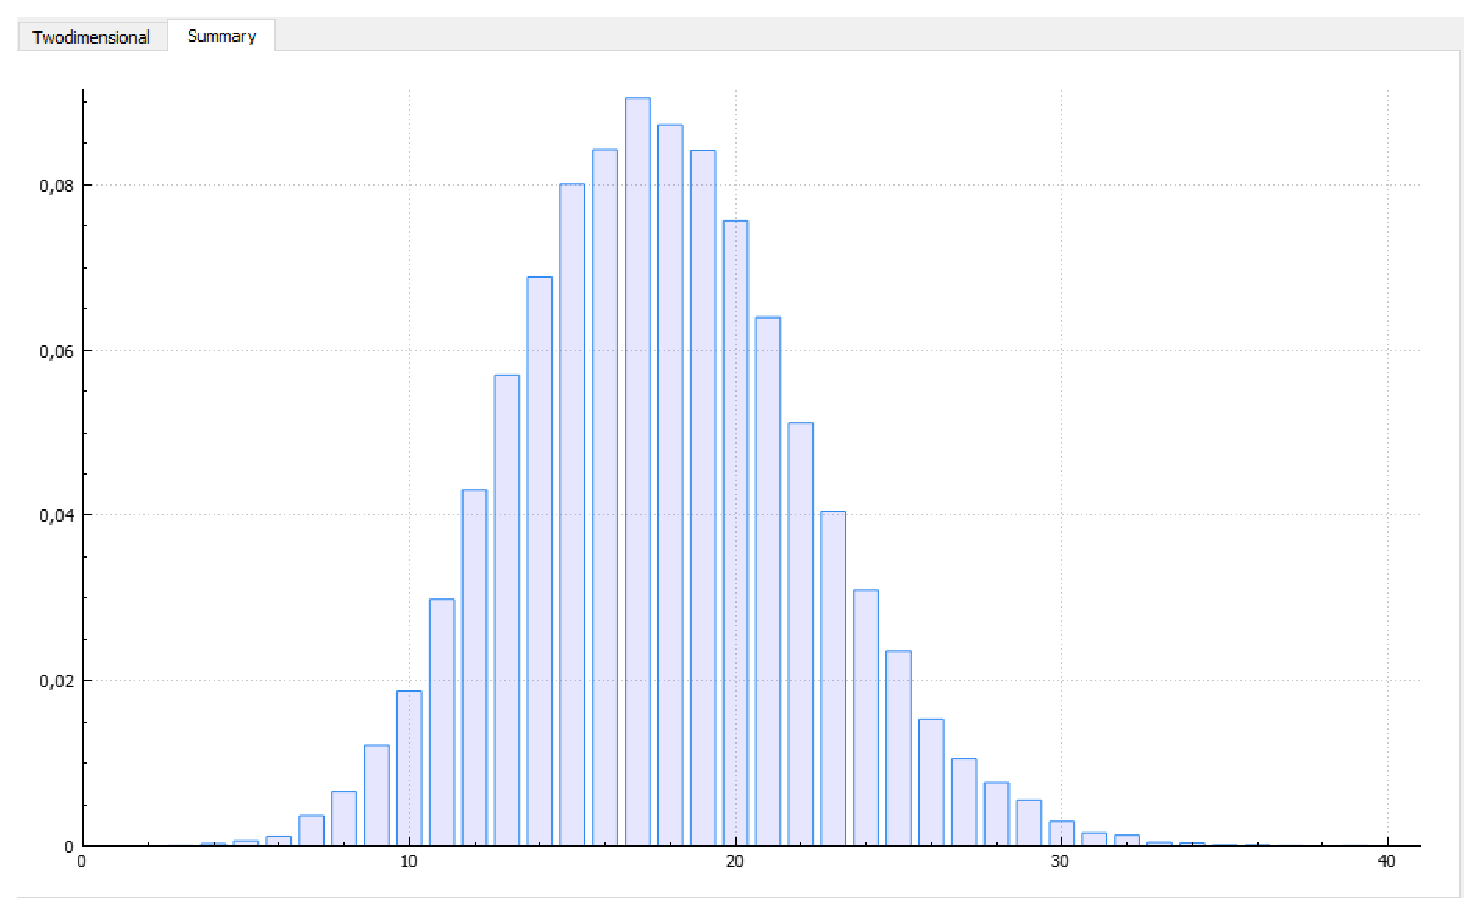
\includegraphics[scale=0.8,width=\textwidth]{interface_mainplot_summary.eps}
	\caption{Вкладка основного графика, отображающая распределение вероятностей суммарного числа обслуженных заявок}
	\label{interface_mainplot_summary}
\end{figure}
\subsubsection{Экспорт результатов моделирования}
В меню Model основного окна имеется опция экспорта в текстовый файл текущего распределения вероятностей числа обслуженных заявок в двумерном виде и суммарном.
\begin{figure}[H]
	\centering
	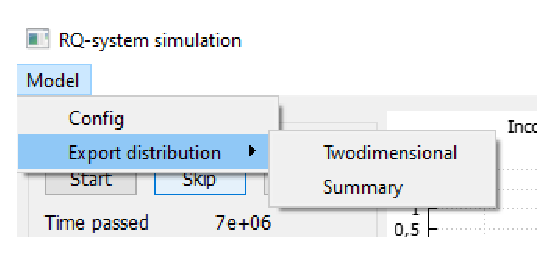
\includegraphics[scale=0.8]{interface_export.eps}
	\caption{Опции экспорта}
	\label{interface_export}
\end{figure}
При выборе опции Summary распределение будет записано в файл формата CSV, где каждое значение будет с новой строки. При выборе опции Twodimensional распределение будет записано в виде таблицы с разделителем, установленным пользователем в окне конфигурации (рисунок \ref{interface_config}). По умолчанию разделителем является символ \textquote{;}. Поскольку формат CSV является основным при работе с данными ввиду удобного табличного представления с помощью разделителей, импортировать и использовать полученные при моделировании данные можно в широком спектре программного обеспечения. Для анализа численных результатов в данной работе используется система компьютерной алгебры Mathcad.
\begin{figure}[H]
	\centering
	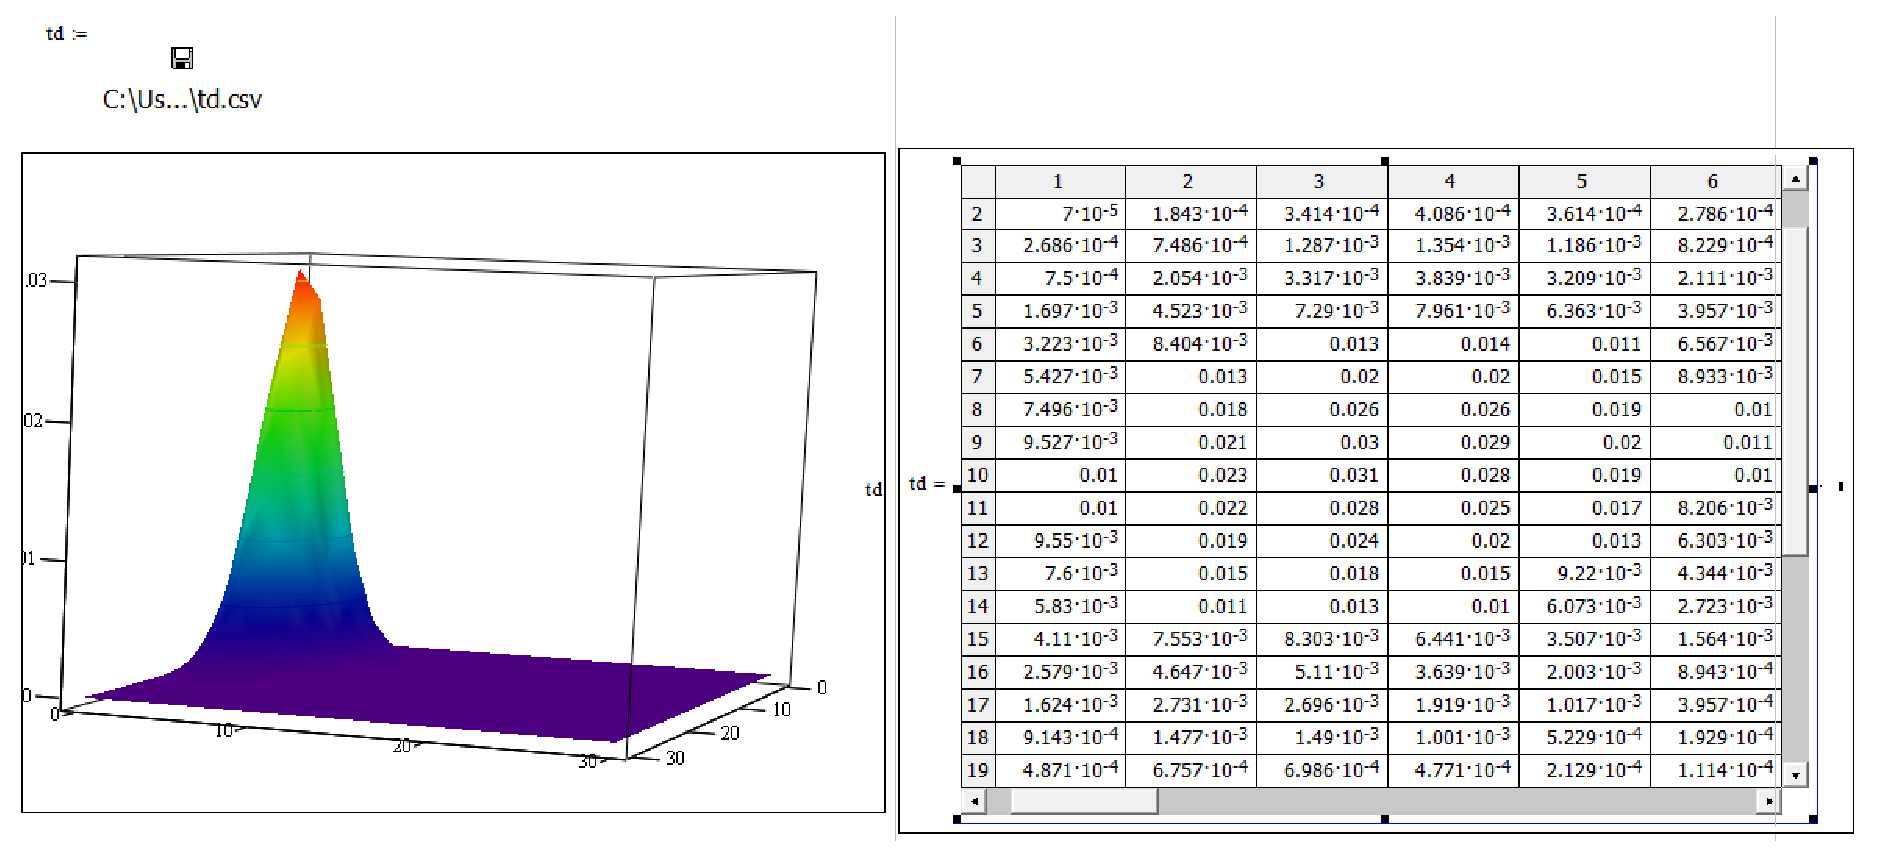
\includegraphics[width=\textwidth]{interface_export_mathcad.eps}
	\caption{Результаты моделирования, импортированные в среду Mathcad}
	\label{interface_export_mathcad}
\end{figure}
На рисунке \ref{interface_export_mathcad} представлена плоскость двумерного распределения вероятностей числа обслуженных заявок (слева) и таблица распределения (справа), полученные в результате моделирования и импорта в среду Mathcad.
\clearpage

\subsection{Особенности реализации}
Реализация предметной области программы выполнена на языке программирования C++ стандарта 2017 года (C++1z). Оболочка программы и графический интерфейс были выполнены на базе фреймворка для разработки кроссплатформенного программного обеспечения QT \cite{QtDoc}. Таким образом, представленная программа является кроссплатформенной, то есть, может быть собрана для работы в операционных системах GNU/Linux, Microsoft Windows и macOS. Выбор в сторону разработки на C++ был сделан, в первую очередь, из--за низкоуровневого программирования, которое позволяет писать эффективный код и более точно распоряжаться используемыми ресурсами системы. По этой же причине, C++ отлично подходит для работы с графикой. Также, в C++ поддерживается объектно--ориентированный подход к программированию, что важно для реализации ранее описанной предметной области программы.
\\\\
Минимальные системные требования для работы программы:
\begin{itemize}
	\item Процессор с тактовой частотой 1.8 ГГц и выше.
	\item Оперативная память емкостью 2 Гб и больше.
	\item Видеоадаптер и монитор VGA с разрешением 1280 х 1024 и выше.
	\item 50 Мб свободного места на диске
	\item Клавиатура и мышь
	\end{itemize}

\subsubsection{Генерация псевдослучайных чисел}
Поскольку генераторы псевдослучайных чисел во многих языках программирования, в том числе, в C++ генерируют новые значения на основе системного времени или такта процессора, возникает проблема повторения последовательности значений при частой генерации, например, в цикле. А поскольку для расчета экспоненциальной задержки каждого события в модели используется генерация случайных чисел, возникновение этой проблемы неизбежно.

Решением проблемы стало использование вихря Мерсенна --- генератора псевдослучайных чисел, основывающимся на свойствах простых числе Мерсенна. Данный генератор лишен многих недостатков других генераторов, таких как предсказуемость, малый период и легко выявляемые статистические закономерности.

В С++ данный алгоритм имеет реализацию под названием MT19937 и содержится в стандартной библиотеке, начиная со стандарта C++11. Его период составляет $2^{19937}$, чего с излишком хватит для продолжительного процесса моделирования. 

В коде использование вихря Мерсенна представлено следующим образом
\begin{lstlisting}
#include <random>

std::random_device rd;
std::mt19937 gen(rd());
std::uniform_real_distribution<double> distribution(0,1);

double NextDouble()
{
	return distribution(gen) ;
}
\end{lstlisting}

\subsubsection{Отображение статуса при ускоренном моделировании}
При ускоренном моделировании возникает проблема отображения статуса моделирования без блокировки основа потока, в котором производится отрисовка графического интерфейса. Проблема заключается в том, что цикл, в котором производится моделирование системы блокирует отрисовку графического интерфейса до окончания его работы, а все объекты графического интерфейса должны находится в основном потоке программы, что исключает создание параллельного потока для отрисовки. Так, пользователь не может удостовериться, что программа продолжает свою работу, ибо процесс перестает отвечать на сигналы операционной системы.
\begin{lstlisting}
class MainWindow : public QMainWindow
{
	...
	private:
	...
	QFutureWatcher<void> watcher;
	...
};
\end{lstlisting}
\begin{lstlisting}
void MainWindow::skip()
{
 if(Environment::Time()>0  && !Environment::isFinished()){
 ...
 timer->stop();
 skipping = true;
 QFuture<void> future = QtConcurrent::run([this]{
	while (!Environment::isFinished() && skipping){
		Environment::NextMoment();
	}
 });
 watcher.setFuture(future);
 progressDialog.exec();
 }
}
\end{lstlisting}

Для решения данной проблемы был использован специальный инструмент фреймворка QT --- QTConcurrent, предназначенный для параллельного запуска ресурсоёмких задач. Так, основной поток будет занят отрисовкой статуса моделирования (рисунок \ref{interface_skip}), а моделирование будет происходить асинхронно, что положительно скажется на быстродействии.
\begin{lstlisting}
connect(&watcher,&QFutureWatcher<void>::finished,this,[=](){
	progressDialog.close();
	updateTime();
});
\end{lstlisting}
Для уведомления модального окна об окончании цикла моделирования служит объект QFutureWatcher, который осуществляет привязку события завершения работы потока к лямбда--функции, в которой производится закрытие окна статуса и обновление отображаемой статистики.
\clearpage